\documentclass[aspectratio=169,11pt]{beamer}
\usetheme{metropolis}
\usepackage{appendixnumberbeamer}
\usepackage{amsmath,amssymb}
\usepackage{xcolor}
\usepackage{booktabs}
\usepackage{tikz}
\usetikzlibrary{arrows.meta,positioning}

% Course palette (mirrors preamble.sty; Beamer needs theme colors set here)
\definecolor{Ink}{HTML}{1B2A4A}
\definecolor{Accent}{HTML}{8C4F2B}
\setbeamercolor{frametitle}{bg=Ink,fg=white}
\setbeamercolor{progress bar}{fg=Accent}
\setbeamercolor{alerted text}{fg=Accent}

\title{Quantifying Information Flow with Entropy}
\subtitle{Module Q32 \textendash\ AI Course 2026}
\author{\textsc{Kukla}}
\institute{Anchor: L2.1 \textbullet\ Week 4}
\date{}

\begin{document}
\maketitle

\begin{frame}{The question hides three questions}
``Can we quantify the information flowing through a model?''
\begin{enumerate}
  \item<1-> \alert{Output uncertainty} --- entropy of $p(x_t\mid x_{<t})$.
    \hfill\textit{exact, cheap}
  \item<2-> \alert{Compression quality} --- bits/token = cross-entropy.
    \hfill\textit{= the training loss}
  \item<3-> \alert{Internal flow} --- mutual information between activations.
    \hfill\textit{careful!}
\end{enumerate}
\vspace{1em}
\onslide<4->{\centering\color{Accent}\textbf{Yes} for 1 \& 2 exactly ---
``yes, carefully'' for 3.}
\end{frame}

\begin{frame}{Entropy: how much is the model hedging?}
For next-token distribution $p$ over vocabulary $\mathcal V$:
\[
  H(p) = -\sum_{v} p(v)\log_2 p(v)\quad\text{bits}
\]
\begin{itemize}
  \item $H=0$: certain. $\quad H=\log_2|\mathcal V|\approx 15$--$17$: uniform guess.
  \item A per-step read-out of confidence --- \emph{after} temperature \& softmax.
  \item High entropy at a decision-critical token $=$ the model is uncertain
    (\emph{after calibration}, a useful abstention flag --- not a correctness oracle).
\end{itemize}
\end{frame}

\begin{frame}{Cross-entropy = the loss = compression}
\[
  \mathrm{CE} = -\tfrac{1}{T}\sum_t \log_2 p_\theta(x_t\mid x_{<t}),
  \qquad \mathrm{PPL}=2^{\mathrm{CE}}
\]
\[
  \mathrm{CE} = \underbrace{H(p_{\text{data}})}_{\text{irreducible}}
  + \underbrace{D_{\mathrm{KL}}(p_{\text{data}}\|p_\theta)}_{\text{what training removes}}
\]
\begin{alertblock}{Compression is literal}
A frozen LLM used as the probability model inside an arithmetic coder beats
\texttt{gzip} on text \emph{and} images (Del\'etang et al.\ 2023).
Bits/token and model quality are one axis.
\end{alertblock}
\end{frame}

\begin{frame}{Three things entropy buys you}
\begin{columns}[T]
\column{0.33\textwidth}
\textbf{Confidence signal}\\[4pt]
High entropy $\to$ abstain / flag hallucination (Q10--Q12).
\column{0.33\textwidth}
\textbf{Decoding}\\[4pt]
Temperature, top-$k$, nucleus, min-$p$ are all entropy-reshaping.
Watch for RL ``entropy collapse.''
\column{0.33\textwidth}
\textbf{Training diagnostic}\\[4pt]
Mean entropy falls from $\sim$16 bits to a few as the model learns.
\end{columns}
\end{frame}

\begin{frame}{Internal flow: the seductive, dangerous part}
Mutual information between a hidden rep $Z=f_\ell(X)$ and input/label:
\[
  I(X;Z) = H(X)-H(X\mid Z)
\]
\begin{center}
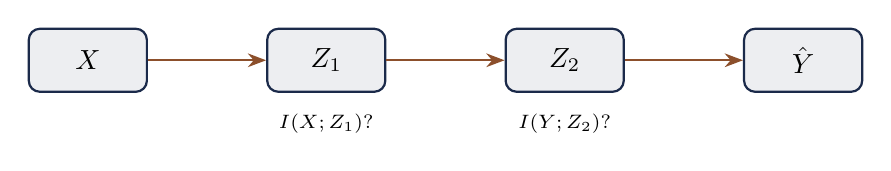
\begin{tikzpicture}[node distance=1.1cm and 1.5cm,
  box/.style={draw=Ink,thick,rounded corners,minimum width=1.5cm,minimum height=0.8cm,fill=Ink!8}]
  \node[box] (x) {$X$};
  \node[box,right=of x] (z1) {$Z_1$};
  \node[box,right=of z1] (z2) {$Z_2$};
  \node[box,right=of z2] (y) {$\hat Y$};
  \draw[-{Stealth},Accent,thick] (x)--(z1);
  \draw[-{Stealth},Accent,thick] (z1)--(z2);
  \draw[-{Stealth},Accent,thick] (z2)--(y);
  \node[below=0.15cm of z1,font=\scriptsize] {$I(X;Z_1)?$};
  \node[below=0.15cm of z2,font=\scriptsize] {$I(Y;Z_2)?$};
\end{tikzpicture}
\end{center}
The Information Bottleneck claimed a ``compression phase.'' \alert{It was mostly a binning artefact.}
\end{frame}

\begin{frame}{The cautionary tale}
\begin{alertblock}{Saxe et al.\ 2018}
The famous IB ``compression phase'' depends on the \emph{nonlinearity} and the
\emph{binning}: \texttt{tanh} shows it, \texttt{ReLU} often doesn't.
For a deterministic net, $I(Z;X)$ is ill-defined/infinite with continuous $X$ (bounded
by $H(X)$ when discrete) --- the plotted number is a property of your \emph{estimator},
not the network.
\end{alertblock}
\centering\color{Accent}\textbf{The estimator \emph{is} the measurement.}
\end{frame}

\begin{frame}{What is actually safe to measure}
\begin{itemize}
  \item \textbf{Attention entropy} --- weights are already a distribution.
    Low $=$ ``pointing'', high $=$ ``averaging''. Exact, no assumptions.
  \item \textbf{Predictive / cross-entropy} --- exact, cheap, load-bearing.
  \item \textbf{MI between activations} --- needs a principled bound (KSG, MINE,
    InfoNCE) and is loose above a few nats.
  \item \textbf{Causal flow?} Don't estimate --- \alert{intervene}: patch/ablate
    the path, measure the output change (Q14/Q27).
\end{itemize}
\end{frame}

\begin{frame}{Takeaways}
\begin{enumerate}
  \item Predictive entropy + perplexity give you most of what you want, exactly.
  \item Attention entropy is a safe internal read-out.
  \item Treat any ``information plane'' plot as a claim about the estimator.
  \item For causal flow, patch --- don't estimate.
\end{enumerate}
\vspace{0.8em}
\centering\small\color{Accent} Code demo: \texttt{entropy\_flow.py} computes all the
safe quantities on \emph{synthetic} distributions (numpy-only, deterministic) ---
same math as a real model --- and shows the binning artefact live.
\end{frame}

\end{document}
